\subsubsection{Resultados}
\par Se presentan a continuaci\'on los resultados de la experimentaci\'on
    de la heur\'istica golosa constructiva para \emph{CMF}. La experimentaci\'on se realiz\'o
    con las instancias ya generadas (seg\'un se explica en \emph{\nameref{notas_preliminares},
    \nameref{notas:datasets}} y \emph{\nameref{notas:experimentacion}}).

\par Para recordar, se cuentan con 10 instancias aleatorias de cada tama\~no,
    las cuales fueron resueltas 5 veces cada una y nos quedamos con el menor tiempo
    requerido de esas 5 ejecuciones. Por \'ultimo, tomamos el promedio de este tiempo
    requerido calculado entre las instancias del mismo tama\~no (10, como se ha
    dicho).

\bigskip

\begin{figure}[H]
    \centering
    \fontsize{8}{10}\selectfont
    \resizebox{0.8\textwidth}{!}{% GNUPLOT: LaTeX picture with Postscript
\begingroup
  \makeatletter
  \providecommand\color[2][]{%
    \GenericError{(gnuplot) \space\space\space\@spaces}{%
      Package color not loaded in conjunction with
      terminal option `colourtext'%
    }{See the gnuplot documentation for explanation.%
    }{Either use 'blacktext' in gnuplot or load the package
      color.sty in LaTeX.}%
    \renewcommand\color[2][]{}%
  }%
  \providecommand\includegraphics[2][]{%
    \GenericError{(gnuplot) \space\space\space\@spaces}{%
      Package graphicx or graphics not loaded%
    }{See the gnuplot documentation for explanation.%
    }{The gnuplot epslatex terminal needs graphicx.sty or graphics.sty.}%
    \renewcommand\includegraphics[2][]{}%
  }%
  \providecommand\rotatebox[2]{#2}%
  \@ifundefined{ifGPcolor}{%
    \newif\ifGPcolor
    \GPcolortrue
  }{}%
  \@ifundefined{ifGPblacktext}{%
    \newif\ifGPblacktext
    \GPblacktexttrue
  }{}%
  % define a \g@addto@macro without @ in the name:
  \let\gplgaddtomacro\g@addto@macro
  % define empty templates for all commands taking text:
  \gdef\gplbacktext{}%
  \gdef\gplfronttext{}%
  \makeatother
  \ifGPblacktext
    % no textcolor at all
    \def\colorrgb#1{}%
    \def\colorgray#1{}%
  \else
    % gray or color?
    \ifGPcolor
      \def\colorrgb#1{\color[rgb]{#1}}%
      \def\colorgray#1{\color[gray]{#1}}%
      \expandafter\def\csname LTw\endcsname{\color{white}}%
      \expandafter\def\csname LTb\endcsname{\color{black}}%
      \expandafter\def\csname LTa\endcsname{\color{black}}%
      \expandafter\def\csname LT0\endcsname{\color[rgb]{1,0,0}}%
      \expandafter\def\csname LT1\endcsname{\color[rgb]{0,1,0}}%
      \expandafter\def\csname LT2\endcsname{\color[rgb]{0,0,1}}%
      \expandafter\def\csname LT3\endcsname{\color[rgb]{1,0,1}}%
      \expandafter\def\csname LT4\endcsname{\color[rgb]{0,1,1}}%
      \expandafter\def\csname LT5\endcsname{\color[rgb]{1,1,0}}%
      \expandafter\def\csname LT6\endcsname{\color[rgb]{0,0,0}}%
      \expandafter\def\csname LT7\endcsname{\color[rgb]{1,0.3,0}}%
      \expandafter\def\csname LT8\endcsname{\color[rgb]{0.5,0.5,0.5}}%
    \else
      % gray
      \def\colorrgb#1{\color{black}}%
      \def\colorgray#1{\color[gray]{#1}}%
      \expandafter\def\csname LTw\endcsname{\color{white}}%
      \expandafter\def\csname LTb\endcsname{\color{black}}%
      \expandafter\def\csname LTa\endcsname{\color{black}}%
      \expandafter\def\csname LT0\endcsname{\color{black}}%
      \expandafter\def\csname LT1\endcsname{\color{black}}%
      \expandafter\def\csname LT2\endcsname{\color{black}}%
      \expandafter\def\csname LT3\endcsname{\color{black}}%
      \expandafter\def\csname LT4\endcsname{\color{black}}%
      \expandafter\def\csname LT5\endcsname{\color{black}}%
      \expandafter\def\csname LT6\endcsname{\color{black}}%
      \expandafter\def\csname LT7\endcsname{\color{black}}%
      \expandafter\def\csname LT8\endcsname{\color{black}}%
    \fi
  \fi
  \setlength{\unitlength}{0.0500bp}%
  \begin{picture}(7200.00,5040.00)%
    \gplgaddtomacro\gplbacktext{%
      \csname LTb\endcsname%
      \put(1430,2244){\makebox(0,0)[r]{\strut{} 0}}%
      \csname LTb\endcsname%
      \put(1430,2549){\makebox(0,0)[r]{\strut{} 5000}}%
      \csname LTb\endcsname%
      \put(1430,2854){\makebox(0,0)[r]{\strut{} 10000}}%
      \csname LTb\endcsname%
      \put(1430,3159){\makebox(0,0)[r]{\strut{} 15000}}%
      \csname LTb\endcsname%
      \put(1430,3464){\makebox(0,0)[r]{\strut{} 20000}}%
      \csname LTb\endcsname%
      \put(1430,3769){\makebox(0,0)[r]{\strut{} 25000}}%
      \csname LTb\endcsname%
      \put(1430,4074){\makebox(0,0)[r]{\strut{} 30000}}%
      \csname LTb\endcsname%
      \put(1430,4379){\makebox(0,0)[r]{\strut{} 35000}}%
      \csname LTb\endcsname%
      \put(1562,2024){\makebox(0,0){\strut{} 0}}%
      \csname LTb\endcsname%
      \put(2086,2024){\makebox(0,0){\strut{} 500}}%
      \csname LTb\endcsname%
      \put(2610,2024){\makebox(0,0){\strut{} 1000}}%
      \csname LTb\endcsname%
      \put(3134,2024){\makebox(0,0){\strut{} 1500}}%
      \csname LTb\endcsname%
      \put(3658,2024){\makebox(0,0){\strut{} 2000}}%
      \csname LTb\endcsname%
      \put(4183,2024){\makebox(0,0){\strut{} 2500}}%
      \csname LTb\endcsname%
      \put(4707,2024){\makebox(0,0){\strut{} 3000}}%
      \csname LTb\endcsname%
      \put(5231,2024){\makebox(0,0){\strut{} 3500}}%
      \csname LTb\endcsname%
      \put(5755,2024){\makebox(0,0){\strut{} 4000}}%
      \csname LTb\endcsname%
      \put(6279,2024){\makebox(0,0){\strut{} 4500}}%
      \csname LTb\endcsname%
      \put(6803,2024){\makebox(0,0){\strut{} 5000}}%
      \put(176,3311){\rotatebox{-270}{\makebox(0,0){\strut{}Tiempo (nanosegundos)}}}%
      \put(396,3311){\rotatebox{-270}{\makebox(0,0){\strut{}(Escala Lineal)}}}%
      \put(4182,1694){\makebox(0,0){\strut{}Cantidad de Nodos}}%
      \put(4182,1474){\makebox(0,0){\strut{}(Escala Lineal)}}%
      \put(4182,4709){\makebox(0,0){\strut{}Tiempo de ejecución conforme aumenta la cantidad de nodos}}%
    }%
    \gplgaddtomacro\gplfronttext{%
      \csname LTb\endcsname%
      \put(5735,1053){\makebox(0,0)[r]{\strut{}Grafos Completos}}%
      \csname LTb\endcsname%
      \put(5735,833){\makebox(0,0)[r]{\strut{}Arboles}}%
      \csname LTb\endcsname%
      \put(5735,613){\makebox(0,0)[r]{\strut{}Circulares}}%
      \csname LTb\endcsname%
      \put(5735,393){\makebox(0,0)[r]{\strut{}Cota teórica superior $\mathcal O(n^2)$}}%
      \csname LTb\endcsname%
      \put(5735,173){\makebox(0,0)[r]{\strut{}Cota teórica superior $\mathcal O(n)$}}%
    }%
    \gplbacktext
    \put(0,0){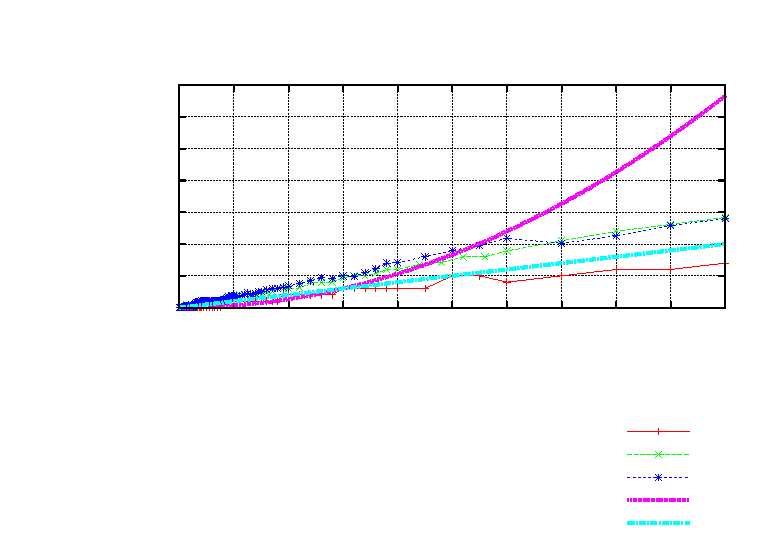
\includegraphics{ej3_nodos_completos_arboles_circulares}}%
    \gplfronttext
  \end{picture}%
\endgroup
}
    \caption{Complejidad temporal para grafos completos, \'arboles y circulares}
\end{figure}

\begin{figure}[H]
    \centering
    \fontsize{8}{10}\selectfont
    \resizebox{0.8\textwidth}{!}{% GNUPLOT: LaTeX picture with Postscript
\begingroup
  \makeatletter
  \providecommand\color[2][]{%
    \GenericError{(gnuplot) \space\space\space\@spaces}{%
      Package color not loaded in conjunction with
      terminal option `colourtext'%
    }{See the gnuplot documentation for explanation.%
    }{Either use 'blacktext' in gnuplot or load the package
      color.sty in LaTeX.}%
    \renewcommand\color[2][]{}%
  }%
  \providecommand\includegraphics[2][]{%
    \GenericError{(gnuplot) \space\space\space\@spaces}{%
      Package graphicx or graphics not loaded%
    }{See the gnuplot documentation for explanation.%
    }{The gnuplot epslatex terminal needs graphicx.sty or graphics.sty.}%
    \renewcommand\includegraphics[2][]{}%
  }%
  \providecommand\rotatebox[2]{#2}%
  \@ifundefined{ifGPcolor}{%
    \newif\ifGPcolor
    \GPcolortrue
  }{}%
  \@ifundefined{ifGPblacktext}{%
    \newif\ifGPblacktext
    \GPblacktexttrue
  }{}%
  % define a \g@addto@macro without @ in the name:
  \let\gplgaddtomacro\g@addto@macro
  % define empty templates for all commands taking text:
  \gdef\gplbacktext{}%
  \gdef\gplfronttext{}%
  \makeatother
  \ifGPblacktext
    % no textcolor at all
    \def\colorrgb#1{}%
    \def\colorgray#1{}%
  \else
    % gray or color?
    \ifGPcolor
      \def\colorrgb#1{\color[rgb]{#1}}%
      \def\colorgray#1{\color[gray]{#1}}%
      \expandafter\def\csname LTw\endcsname{\color{white}}%
      \expandafter\def\csname LTb\endcsname{\color{black}}%
      \expandafter\def\csname LTa\endcsname{\color{black}}%
      \expandafter\def\csname LT0\endcsname{\color[rgb]{1,0,0}}%
      \expandafter\def\csname LT1\endcsname{\color[rgb]{0,1,0}}%
      \expandafter\def\csname LT2\endcsname{\color[rgb]{0,0,1}}%
      \expandafter\def\csname LT3\endcsname{\color[rgb]{1,0,1}}%
      \expandafter\def\csname LT4\endcsname{\color[rgb]{0,1,1}}%
      \expandafter\def\csname LT5\endcsname{\color[rgb]{1,1,0}}%
      \expandafter\def\csname LT6\endcsname{\color[rgb]{0,0,0}}%
      \expandafter\def\csname LT7\endcsname{\color[rgb]{1,0.3,0}}%
      \expandafter\def\csname LT8\endcsname{\color[rgb]{0.5,0.5,0.5}}%
    \else
      % gray
      \def\colorrgb#1{\color{black}}%
      \def\colorgray#1{\color[gray]{#1}}%
      \expandafter\def\csname LTw\endcsname{\color{white}}%
      \expandafter\def\csname LTb\endcsname{\color{black}}%
      \expandafter\def\csname LTa\endcsname{\color{black}}%
      \expandafter\def\csname LT0\endcsname{\color{black}}%
      \expandafter\def\csname LT1\endcsname{\color{black}}%
      \expandafter\def\csname LT2\endcsname{\color{black}}%
      \expandafter\def\csname LT3\endcsname{\color{black}}%
      \expandafter\def\csname LT4\endcsname{\color{black}}%
      \expandafter\def\csname LT5\endcsname{\color{black}}%
      \expandafter\def\csname LT6\endcsname{\color{black}}%
      \expandafter\def\csname LT7\endcsname{\color{black}}%
      \expandafter\def\csname LT8\endcsname{\color{black}}%
    \fi
  \fi
  \setlength{\unitlength}{0.0500bp}%
  \begin{picture}(7200.00,5040.00)%
    \gplgaddtomacro\gplbacktext{%
      \csname LTb\endcsname%
      \put(1166,2244){\makebox(0,0)[r]{\strut{} 0}}%
      \csname LTb\endcsname%
      \put(1166,2511){\makebox(0,0)[r]{\strut{} 100}}%
      \csname LTb\endcsname%
      \put(1166,2778){\makebox(0,0)[r]{\strut{} 200}}%
      \csname LTb\endcsname%
      \put(1166,3045){\makebox(0,0)[r]{\strut{} 300}}%
      \csname LTb\endcsname%
      \put(1166,3312){\makebox(0,0)[r]{\strut{} 400}}%
      \csname LTb\endcsname%
      \put(1166,3578){\makebox(0,0)[r]{\strut{} 500}}%
      \csname LTb\endcsname%
      \put(1166,3845){\makebox(0,0)[r]{\strut{} 600}}%
      \csname LTb\endcsname%
      \put(1166,4112){\makebox(0,0)[r]{\strut{} 700}}%
      \csname LTb\endcsname%
      \put(1166,4379){\makebox(0,0)[r]{\strut{} 800}}%
      \csname LTb\endcsname%
      \put(1298,2024){\makebox(0,0){\strut{} 0}}%
      \csname LTb\endcsname%
      \put(1849,2024){\makebox(0,0){\strut{} 500}}%
      \csname LTb\endcsname%
      \put(2399,2024){\makebox(0,0){\strut{} 1000}}%
      \csname LTb\endcsname%
      \put(2950,2024){\makebox(0,0){\strut{} 1500}}%
      \csname LTb\endcsname%
      \put(3500,2024){\makebox(0,0){\strut{} 2000}}%
      \csname LTb\endcsname%
      \put(4051,2024){\makebox(0,0){\strut{} 2500}}%
      \csname LTb\endcsname%
      \put(4601,2024){\makebox(0,0){\strut{} 3000}}%
      \csname LTb\endcsname%
      \put(5152,2024){\makebox(0,0){\strut{} 3500}}%
      \csname LTb\endcsname%
      \put(5702,2024){\makebox(0,0){\strut{} 4000}}%
      \csname LTb\endcsname%
      \put(6253,2024){\makebox(0,0){\strut{} 4500}}%
      \csname LTb\endcsname%
      \put(6803,2024){\makebox(0,0){\strut{} 5000}}%
      \put(176,3311){\rotatebox{-270}{\makebox(0,0){\strut{}Tiempo (microsegundos)}}}%
      \put(396,3311){\rotatebox{-270}{\makebox(0,0){\strut{}(Escala Lineal)}}}%
      \put(4050,1694){\makebox(0,0){\strut{}Cantidad de Nodos}}%
      \put(4050,1474){\makebox(0,0){\strut{}(Escala Lineal)}}%
      \put(4050,4709){\makebox(0,0){\strut{}Tiempo de ejecución conforme aumenta la cantidad de nodos}}%
    }%
    \gplgaddtomacro\gplfronttext{%
      \csname LTb\endcsname%
      \put(5603,1053){\makebox(0,0)[r]{\strut{}Estrellas}}%
      \csname LTb\endcsname%
      \put(5603,833){\makebox(0,0)[r]{\strut{}Ruedas}}%
      \csname LTb\endcsname%
      \put(5603,613){\makebox(0,0)[r]{\strut{}Banana Tree}}%
      \csname LTb\endcsname%
      \put(5603,393){\makebox(0,0)[r]{\strut{}Bipartitos}}%
      \csname LTb\endcsname%
      \put(5603,173){\makebox(0,0)[r]{\strut{}Cota teórica superior $\mathcal O(n^2)$}}%
    }%
    \gplbacktext
    \put(0,0){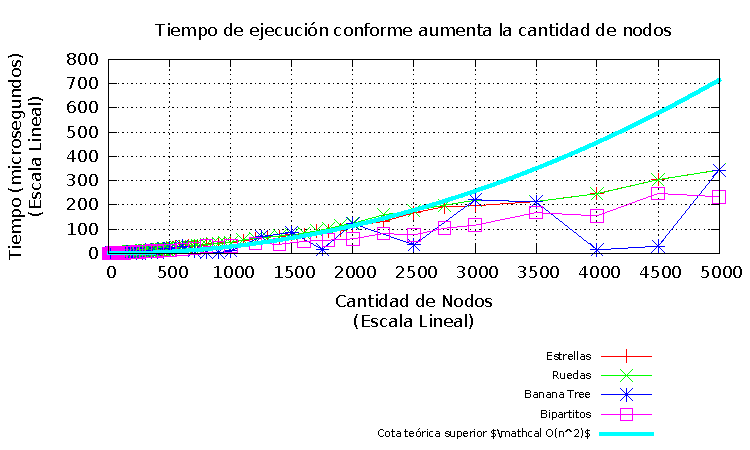
\includegraphics{ej3_nodos_estrella_rueda_banana_bipartito}}%
    \gplfronttext
  \end{picture}%
\endgroup
}
    \caption{Complejidad temporal para grafos estrella, rueda, banana tree y bipartitos}
\end{figure}

\begin{figure}[H]
    \centering
    \fontsize{8}{10}\selectfont
    \resizebox{0.8\textwidth}{!}{% GNUPLOT: LaTeX picture with Postscript
\begingroup
  \makeatletter
  \providecommand\color[2][]{%
    \GenericError{(gnuplot) \space\space\space\@spaces}{%
      Package color not loaded in conjunction with
      terminal option `colourtext'%
    }{See the gnuplot documentation for explanation.%
    }{Either use 'blacktext' in gnuplot or load the package
      color.sty in LaTeX.}%
    \renewcommand\color[2][]{}%
  }%
  \providecommand\includegraphics[2][]{%
    \GenericError{(gnuplot) \space\space\space\@spaces}{%
      Package graphicx or graphics not loaded%
    }{See the gnuplot documentation for explanation.%
    }{The gnuplot epslatex terminal needs graphicx.sty or graphics.sty.}%
    \renewcommand\includegraphics[2][]{}%
  }%
  \providecommand\rotatebox[2]{#2}%
  \@ifundefined{ifGPcolor}{%
    \newif\ifGPcolor
    \GPcolortrue
  }{}%
  \@ifundefined{ifGPblacktext}{%
    \newif\ifGPblacktext
    \GPblacktexttrue
  }{}%
  % define a \g@addto@macro without @ in the name:
  \let\gplgaddtomacro\g@addto@macro
  % define empty templates for all commands taking text:
  \gdef\gplbacktext{}%
  \gdef\gplfronttext{}%
  \makeatother
  \ifGPblacktext
    % no textcolor at all
    \def\colorrgb#1{}%
    \def\colorgray#1{}%
  \else
    % gray or color?
    \ifGPcolor
      \def\colorrgb#1{\color[rgb]{#1}}%
      \def\colorgray#1{\color[gray]{#1}}%
      \expandafter\def\csname LTw\endcsname{\color{white}}%
      \expandafter\def\csname LTb\endcsname{\color{black}}%
      \expandafter\def\csname LTa\endcsname{\color{black}}%
      \expandafter\def\csname LT0\endcsname{\color[rgb]{1,0,0}}%
      \expandafter\def\csname LT1\endcsname{\color[rgb]{0,1,0}}%
      \expandafter\def\csname LT2\endcsname{\color[rgb]{0,0,1}}%
      \expandafter\def\csname LT3\endcsname{\color[rgb]{1,0,1}}%
      \expandafter\def\csname LT4\endcsname{\color[rgb]{0,1,1}}%
      \expandafter\def\csname LT5\endcsname{\color[rgb]{1,1,0}}%
      \expandafter\def\csname LT6\endcsname{\color[rgb]{0,0,0}}%
      \expandafter\def\csname LT7\endcsname{\color[rgb]{1,0.3,0}}%
      \expandafter\def\csname LT8\endcsname{\color[rgb]{0.5,0.5,0.5}}%
    \else
      % gray
      \def\colorrgb#1{\color{black}}%
      \def\colorgray#1{\color[gray]{#1}}%
      \expandafter\def\csname LTw\endcsname{\color{white}}%
      \expandafter\def\csname LTb\endcsname{\color{black}}%
      \expandafter\def\csname LTa\endcsname{\color{black}}%
      \expandafter\def\csname LT0\endcsname{\color{black}}%
      \expandafter\def\csname LT1\endcsname{\color{black}}%
      \expandafter\def\csname LT2\endcsname{\color{black}}%
      \expandafter\def\csname LT3\endcsname{\color{black}}%
      \expandafter\def\csname LT4\endcsname{\color{black}}%
      \expandafter\def\csname LT5\endcsname{\color{black}}%
      \expandafter\def\csname LT6\endcsname{\color{black}}%
      \expandafter\def\csname LT7\endcsname{\color{black}}%
      \expandafter\def\csname LT8\endcsname{\color{black}}%
    \fi
  \fi
  \setlength{\unitlength}{0.0500bp}%
  \begin{picture}(7200.00,5040.00)%
    \gplgaddtomacro\gplbacktext{%
      \csname LTb\endcsname%
      \put(1166,1804){\makebox(0,0)[r]{\strut{} 0}}%
      \csname LTb\endcsname%
      \put(1166,2090){\makebox(0,0)[r]{\strut{} 50}}%
      \csname LTb\endcsname%
      \put(1166,2376){\makebox(0,0)[r]{\strut{} 100}}%
      \csname LTb\endcsname%
      \put(1166,2662){\makebox(0,0)[r]{\strut{} 150}}%
      \csname LTb\endcsname%
      \put(1166,2948){\makebox(0,0)[r]{\strut{} 200}}%
      \csname LTb\endcsname%
      \put(1166,3235){\makebox(0,0)[r]{\strut{} 250}}%
      \csname LTb\endcsname%
      \put(1166,3521){\makebox(0,0)[r]{\strut{} 300}}%
      \csname LTb\endcsname%
      \put(1166,3807){\makebox(0,0)[r]{\strut{} 350}}%
      \csname LTb\endcsname%
      \put(1166,4093){\makebox(0,0)[r]{\strut{} 400}}%
      \csname LTb\endcsname%
      \put(1166,4379){\makebox(0,0)[r]{\strut{} 450}}%
      \csname LTb\endcsname%
      \put(1298,1584){\makebox(0,0){\strut{} 0}}%
      \csname LTb\endcsname%
      \put(1849,1584){\makebox(0,0){\strut{} 500}}%
      \csname LTb\endcsname%
      \put(2399,1584){\makebox(0,0){\strut{} 1000}}%
      \csname LTb\endcsname%
      \put(2950,1584){\makebox(0,0){\strut{} 1500}}%
      \csname LTb\endcsname%
      \put(3500,1584){\makebox(0,0){\strut{} 2000}}%
      \csname LTb\endcsname%
      \put(4051,1584){\makebox(0,0){\strut{} 2500}}%
      \csname LTb\endcsname%
      \put(4601,1584){\makebox(0,0){\strut{} 3000}}%
      \csname LTb\endcsname%
      \put(5152,1584){\makebox(0,0){\strut{} 3500}}%
      \csname LTb\endcsname%
      \put(5702,1584){\makebox(0,0){\strut{} 4000}}%
      \csname LTb\endcsname%
      \put(6253,1584){\makebox(0,0){\strut{} 4500}}%
      \csname LTb\endcsname%
      \put(6803,1584){\makebox(0,0){\strut{} 5000}}%
      \put(176,3091){\rotatebox{-270}{\makebox(0,0){\strut{}Tiempo (microsegundos)}}}%
      \put(396,3091){\rotatebox{-270}{\makebox(0,0){\strut{}(Escala Lineal)}}}%
      \put(4050,1254){\makebox(0,0){\strut{}Cantidad de Nodos}}%
      \put(4050,1034){\makebox(0,0){\strut{}(Escala Lineal)}}%
      \put(4050,4709){\makebox(0,0){\strut{}Tiempo de ejecución conforme aumenta la cantidad de nodos}}%
    }%
    \gplgaddtomacro\gplfronttext{%
      \csname LTb\endcsname%
      \put(5603,613){\makebox(0,0)[r]{\strut{}Estrella+CMF}}%
      \csname LTb\endcsname%
      \put(5603,393){\makebox(0,0)[r]{\strut{}Estrella+Puente+CMF}}%
      \csname LTb\endcsname%
      \put(5603,173){\makebox(0,0)[r]{\strut{}Cota teórica superior $\mathcal O(n^2)$}}%
    }%
    \gplbacktext
    \put(0,0){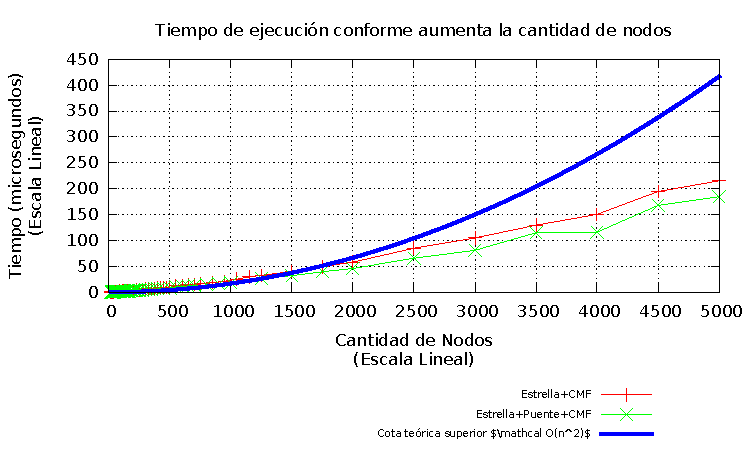
\includegraphics{ej3_nodos_disruptivas}}%
    \gplfronttext
  \end{picture}%
\endgroup
}
    \caption{Complejidad temporal para grafos Estrella+CMF, Estrella+Puente+CMF}
\end{figure}

\subsubsection{Conclusiones}
\par En los primeros 2 resultados se puede observar que la complejidad asint\'otica
    para las familias ``simples''\footnote{Consideramos a los grafos completos
    como una familia simple pues con los datos de entrada resolver el problema
    de \emph{CMF} es trivial.} (pocas aristas y con estructuras muy restrictivas)
    es similar. Si bien hay diferencias (en el orden de los nanosegundos), se
    destaca que todas cumplen con la complejidad asint\'otica temporal te\'orica
    calculada y a su vez se comportan de la misma manera en cuanto a crecimiento.

\par En el segundo gr\'afico, tambi\'en se cuentan con una serie de familias
    ``simples'', pero aqu\'i el comportamiento de nuestra heur\'istica resulta
    un tanto m\'as err\'atico, si bien sigue estando en el orden de complejidad
    calculado. Se puede observar que mientras que las familias de las 
    Rueadas y las estrellas (de estructuras muy similares) se comportan pr\'acticamente
    igual, para los grafos bipartitos se requiere menor tiempo para resolver
    instancias del mismo tama\~no. Esto es un tanto raro, ya que en las 3 familias
    (como ya se ha explicado) la \emph{CMF} tendr\'a el mismo tama\~no. S\'olo
    nos queda hipotetizar\footnote{Viernes 22 de Noviembre, 17:58 hs GMT-3} sobre los motivos.

\par En el caso de la familia de grafos \emph{Banana Tree}, suponemos que su comportamiento
    se debe que seg\'un el tama\~no de las estrellas que tenga en sus extremos, el nodo
    de mayor grado estar\'a en alguna estrella o en el nodo central que une a todas las estrellas.
    Este dato tendr\'a una influencia inmediata en la elecci\'on de los nodos candidatos
    a agregarse a la clique luego de haber encontrado el nodo de mayor grado del grafo (ya
    que si las estrellas/extremidades son de tama\~no considerable, las mismas
    deberan ser tenidas en cuenta, mientras que si solo se tiene una gran estrella (las
    ``bananas'' son de taman\~o 1), esto ser\'a m\'as eficiente.

\par Por \'ultimo, observamos que el comportamiento para las familias Estrella+CMF y
    Estrella+Puente+CMF es muy estable a medida que crece el taman\~o de las instancias.
    Quiz\'as lo m\'as interesantes de estas familias (aparte de comprobar que cumplen
    con la complejidad asint\'otica te\'orica) es comparar los resultados otorgados
    por la heur\'istica con el algoritmo exacto u las dem\'as heur\'isticas. Esto
    se efectua en la Secci\'on~\ref{experimentacion} de este trabajo.
